%Appendix
%%\renewcommand{\thefigure}{A.\arabic{figure}}
\counterwithin{figure}{chapter}
\chapter{Shadow nanowires supplement data} 
\section{Milling test on the tantalum nanowires and tantalum}

The usual way to form contacts on nanowires is using RF milling on the nanowires and then depositing metal on gold and the terminals of nanowires, and this works for both tantalum and aluminum shadow nanowires.   However, since our contacts are aluminum or tantalum along with oxidation layer, we are recommended to use Kaufman milling on the nanowires. We, from previous DC experiment data, know that the aluminum shadow nanowire can withstand 1 minute Kaufman milling and form a good connection to the contact pad. We still need to test whether the tantalum nanowire survived after 1 minute Kaufman milling.
\begin{figure}[h!]
    \centering
    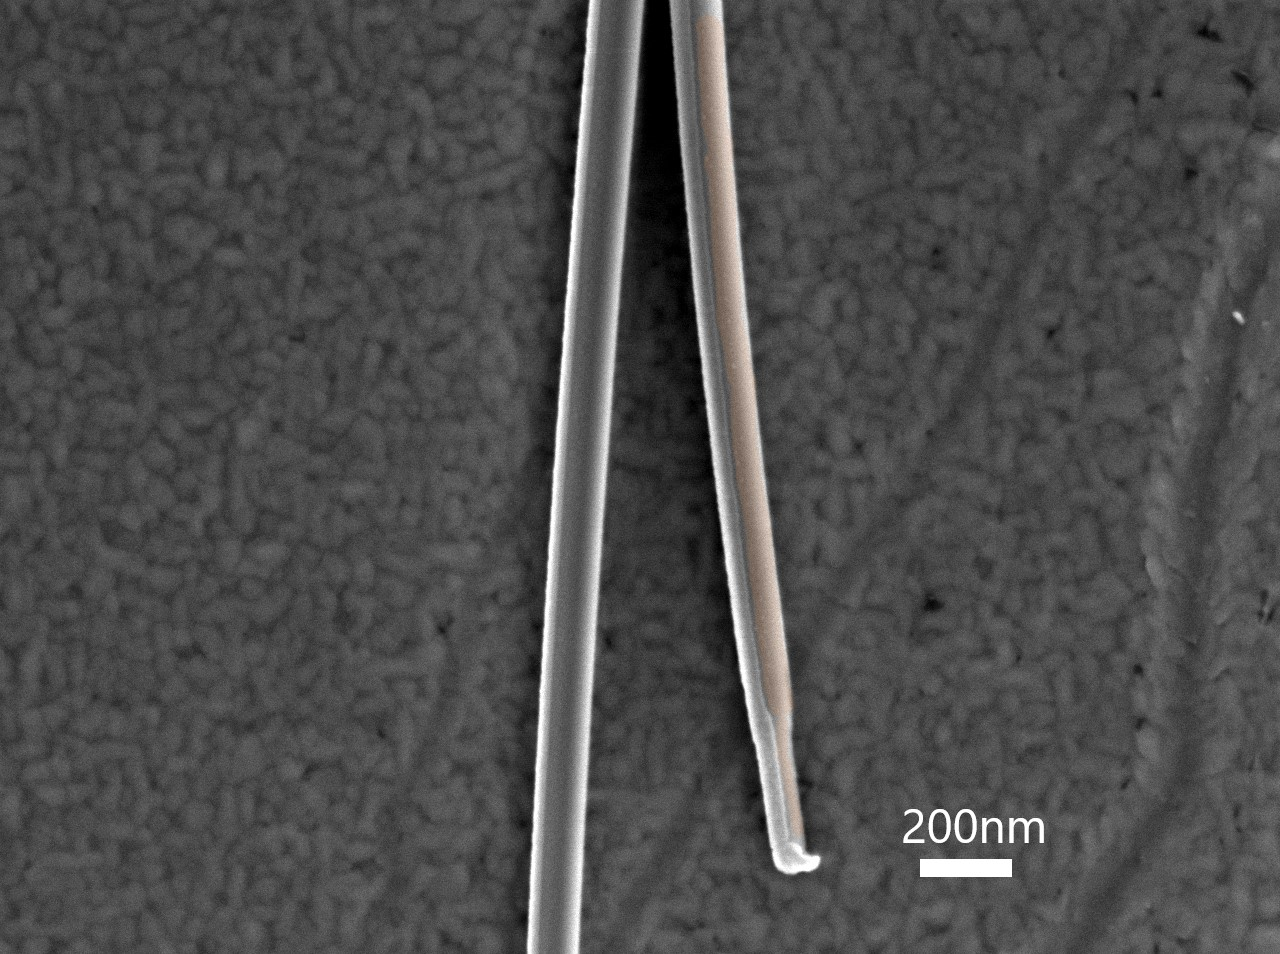
\includegraphics[width=0.7\textwidth]{Pic/Millingtest.jpg}
    \caption{The nanowires after milling. The orange part is the tantalum.}
    \label{fig:my_label}
\end{figure}
The SEM shows that the tantalum nanowires remains visually intact after Kaufman milling. 

The next step is to test whether this milling recipe works for bulk tantalum. We fabricate a chip with deposition metal between the contacts and measure the differential resistance by four terminal measurement of this 'fake' wire in board station (higher than the $T_C$ of $\alpha$-phase tantalum. The chip has in total 3 'fake' aluminum wires. All of them shows tens of Ohm resistance, which means the milling works well on tantalum.  

\begin{figure}[h!]
    \centering
    \begin{subfigure}[b]{0.48\textwidth}
         \centering
        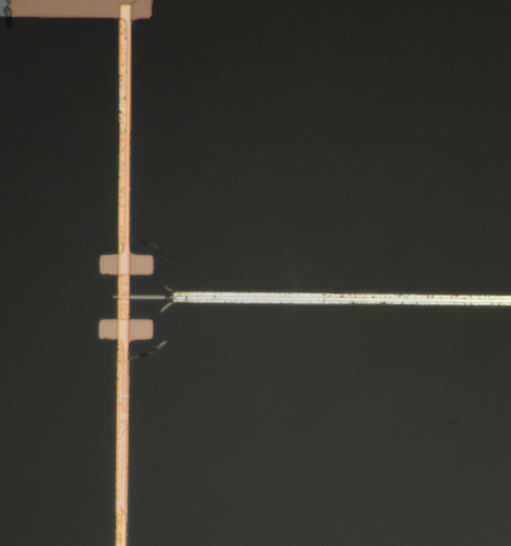
\includegraphics[width=0.98\textwidth]{Pic/Ta_millingtest.png}
        \caption{}
        \label{fig:my_label}
     \end{subfigure}
     \hfill
     \begin{subfigure}[b]{0.48\textwidth}
         \centering
         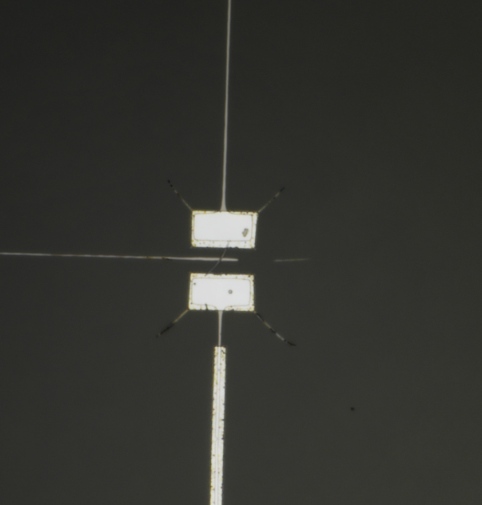
\includegraphics[width=\textwidth]{Pic/Ta_millingtest_Nw.png}
         \caption{}
         \label{}
     \end{subfigure}
     \caption{(a) The 'fake' aluminum nanowire (in orange color) deposited by AJA with bulk Tantalum underneath it. The right metal strip is the gate line, which remains floating when measuring the resistance. (b) The nanowire is linked to the bulk tantalum with aluminum contacts. The crack like aluminum strips around the contacts are because of the exposure problem. We don't use the discharge layer on top for this chip, thus the resist breaks and leaves the strips.}
    \label{Tamilling}
\end{figure}

The real nanowires with (1 of 3) and without (2 of 3) junctions, however, all have a resistance to around 10 $k\Omega$. This is higher than what we are expected because the nanowires without junction is merely acting as a piece of metal. Nevertheless, the measurement data in dilution fridge shows the supercurrent across the junction, which means the line resistance can be eliminated when the metal is under critical temperature. So this high resistance issue remains unsolved and we might test it once again to find out the issue. 

\section{Gate tunability test on tantalum nanowires}

Another important thing to demonstrate is to find out where the junction is gate tunable. This tantalum nanowire is loaded into board station and go through a current bias sweep.
\begin{figure}[h!]
    \begin{subfigure}[b]{0.47\textwidth}
        \centering
        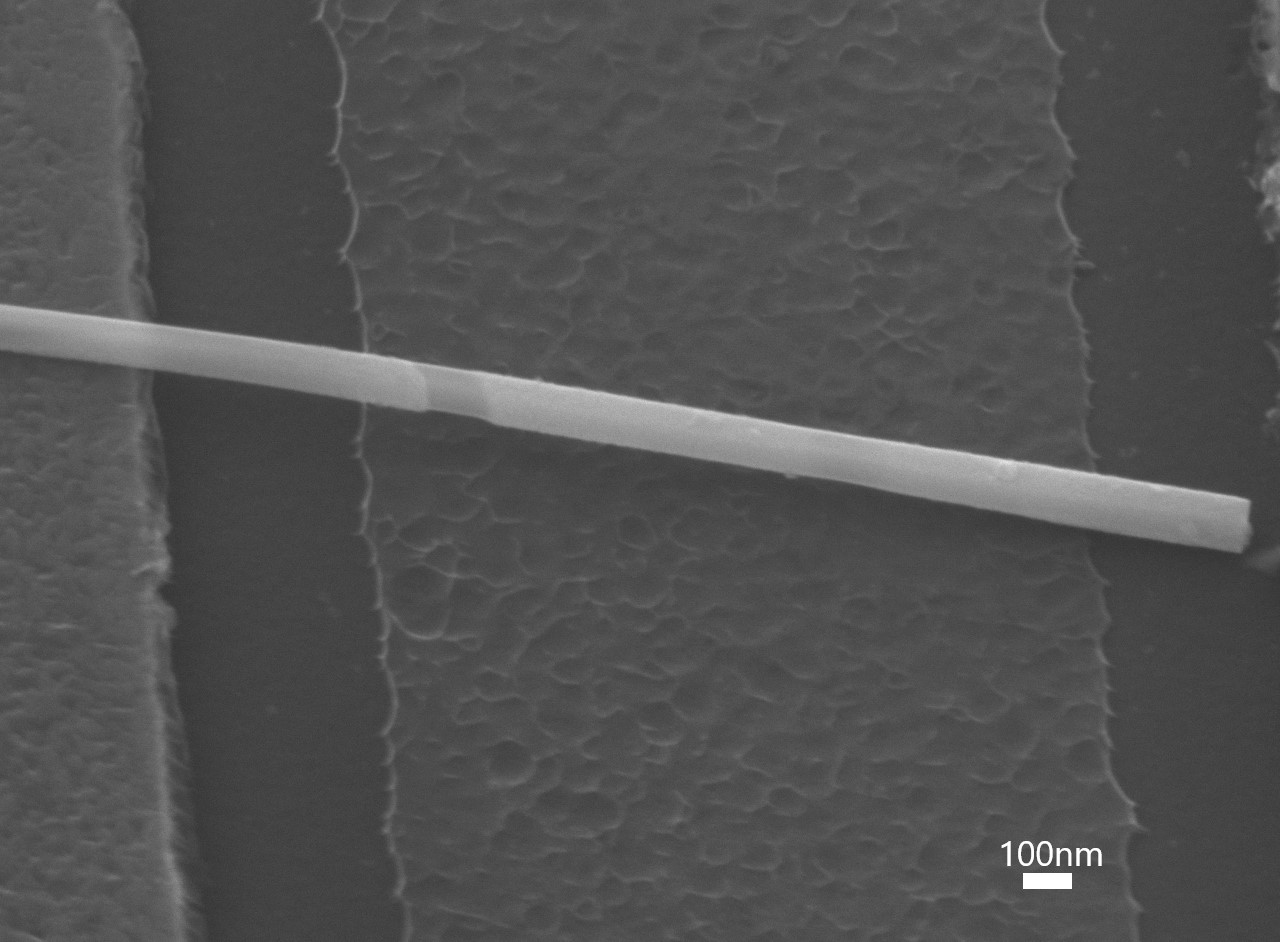
\includegraphics[width=\textwidth]{Pic/GatetestNW.jpg}
        \caption{}
        \label{fig:my_label}
        \end{subfigure}
     \hfill
     \begin{subfigure}[b]{0.51\textwidth}
         \centering
         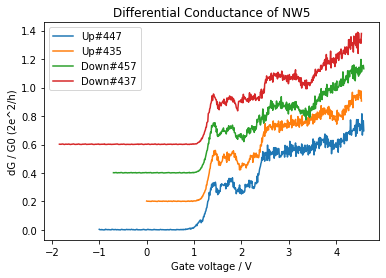
\includegraphics[width=\textwidth]{Pic/Gatetest.png}
         \caption{}
         \label{}
     \end{subfigure}
     \caption{(a) The nanowire and the half-etched bottom gate on the chip. (b) The measured differential resistance with respect to the gate. The line is offset by 0.2 conductance quantum for each.}
     \label{}
\end{figure}
The nanowire is pinch off when no gate voltage is applied, but gradually open after applying positive gate voltage. We conclude in this experiment that the InAs/Ta nanowire is gate tunable and we can use it for DC measurement in dilution fridge. 

\section{Tantalum nanowires supplement data and images}
The measurement are all done through four-terminal connection in dilution fridge
\textbf{Device 1} (Kinky wire shown in the main text): This device is from DC Chip 2 NW7
\begin{figure}[htbp]
    \centering
    \begin{subfigure}[b]{0.49\textwidth}
            \centering
            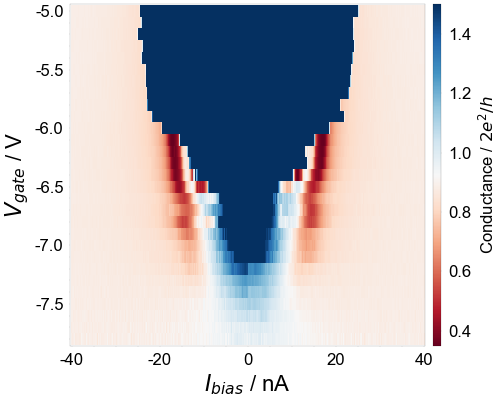
\includegraphics[width=\linewidth]{Pic/KinkyIbiasCond.png}
            \caption{}
            \label{fig:my_label}
     \end{subfigure}
     \hfill
     \begin{subfigure}[b]{0.49\textwidth}
            \centering
            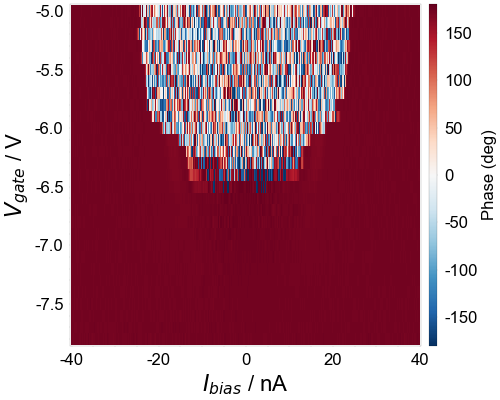
\includegraphics[width=\linewidth]{Pic/KinkyIbiasPhase.png}
            \caption{}
            \label{fig:my_label}
     \end{subfigure}
    \caption{(a) The measured conductance of the kinky wire. (b) The measured phase while biasing with current. This shows that the inner is truly superconducting.}
    \label{Kinkysupp}
\end{figure}
\begin{figure}[h!]
    \centering
    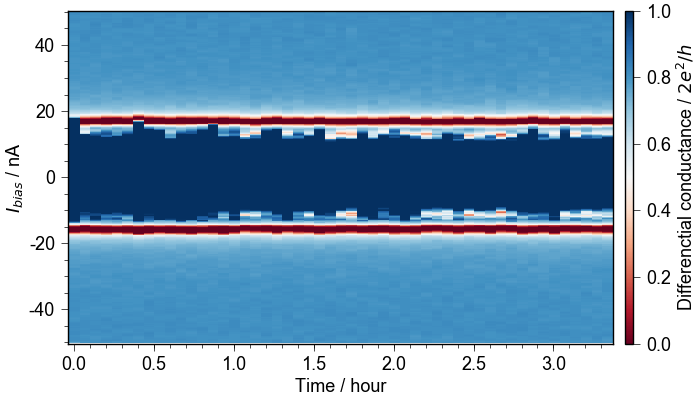
\includegraphics[width=0.8\textwidth]{Pic/KinkySta.png}
    \caption{The stability measurement on the kinky wire for over 3 hours}
    \label{kinkysta}
\end{figure}

\clearpage

\noindent \textbf{Device 2} (straight wire shown in the main text): This device is from DC Chip 6 NW2

\begin{figure}[h!]
    \centering
    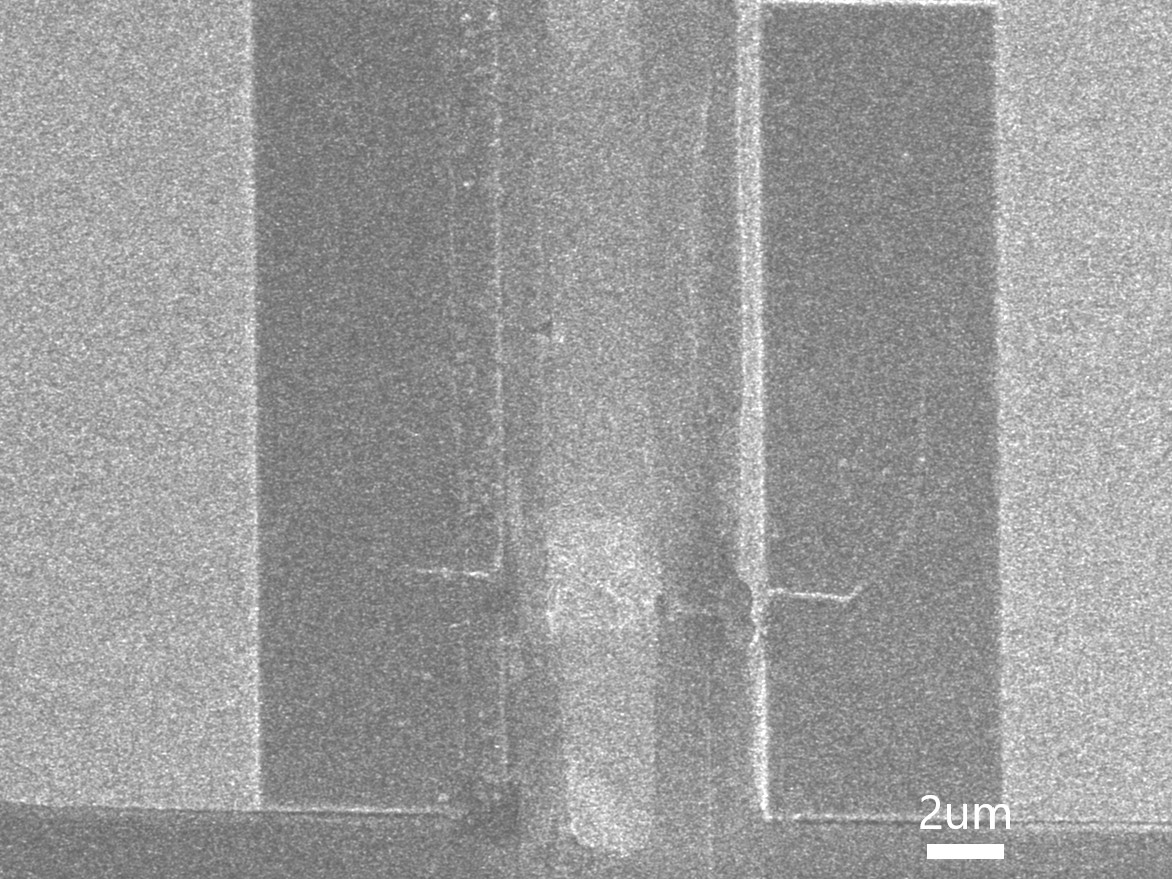
\includegraphics[width=0.7\linewidth]{Pic/NW2SEM.jpg}
    \caption{The nanowire explodes after approximately 2 minutes scan in post-measurement SEM.}
    \label{fig:my_label}
\end{figure}
\begin{figure}[h!]
    \centering
    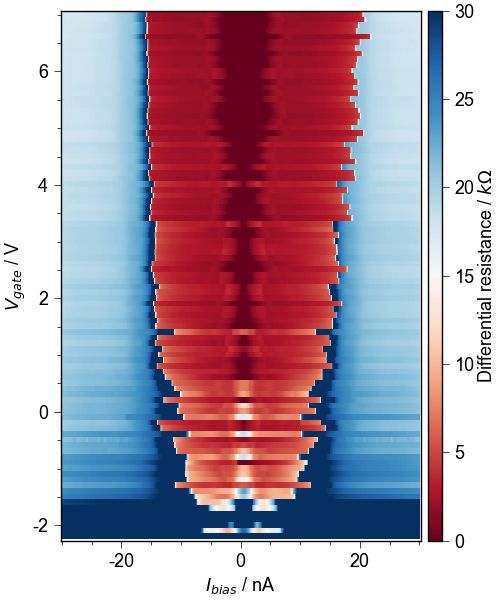
\includegraphics[width=0.6\linewidth]{Pic/D2_Icup.png}
    \caption{The trial to fully open up the junction and get rid of the dot-like behaviour in the junction. The finite resistance still exist inside the critical current regime even the gate voltage goes to 7 V.}
    \label{fig:my_label}
\end{figure}
\clearpage
\noindent \textbf{Device 3}: This device is from DC Chip 2 NW4 (the straight wire 2 in the context)

\begin{figure}[h!]
    \centering
    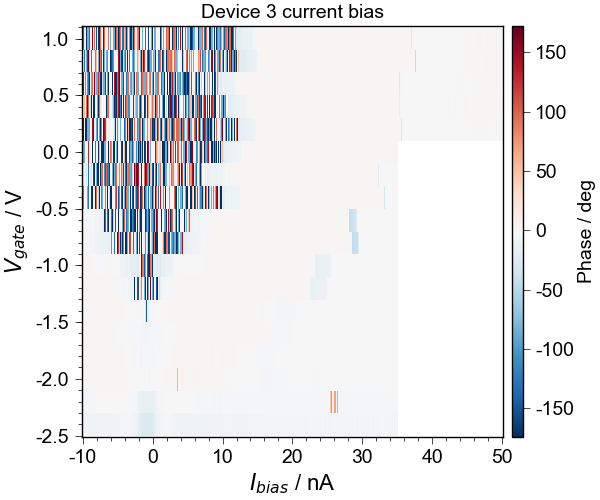
\includegraphics[width=0.8\textwidth]{Pic/D3Ibiasphase.png}
    \caption{Support diagram for Fig \ref{D3 current bias} to show that it is truly superconducting inside the critical current regime}
    \label{fig:my_label}
\end{figure}

\clearpage
\noindent \textbf{Device 4}: This device is from DC Chip 2 NW3

\begin{figure}[h!]
    \centering
    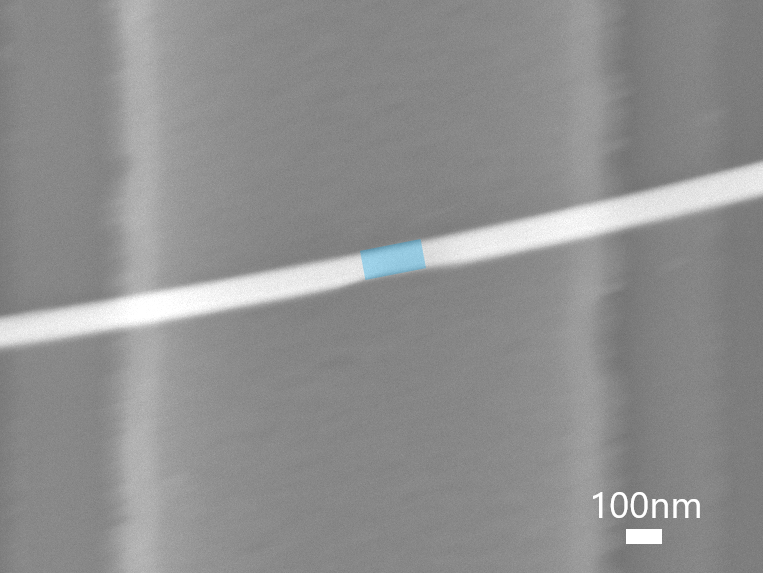
\includegraphics[width=0.7\textwidth]{Pic/D4.png}r
    \caption{The nanowire overview in the SEM after transferring}
    \label{fig:my_label}
\end{figure}

\begin{figure}[h!]
    \centering
    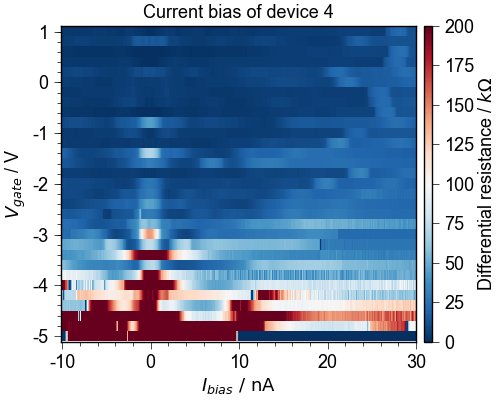
\includegraphics[width=0.8\textwidth]{Pic/D4_Ibias.png}
    \caption{Current bias measurement of device 4. The device's differential resistance inside the critical current regime seems very noisy and mostly has no supercurrent flowing through while applying small current bias.}
    \label{fig:my_label}
\end{figure}

\chapter{Tantalum etch test on Electron beam lithography}
\counterwithin{figure}{chapter}

One major difficulty on the nano-scale Tantalum wet etch by EBL is the e-beam resist are on data sheet, less compatible to hydrofluoric acid and nitric acid. Success on etching in buffered HF (1:10) by using Csar 62 (https://www.allresist.com/resist-wiki-boe-etching-of-sio2-with-csar-62-mask/) and cold buffered HF (1:20) by PMMA A2 is reported and although the resist wiki on Allresist shows concentrated oxidation acid like nitric acid acts as a remover on E-beam resist already at room temperature (https://www.allresist.com/resist-wiki-how-high-is-the-etch-resistance-of-e-beam-resists-in-the-presence-of-strong-acids), we want to try if the resist can survive until the Tantalum is fully etched.
\section{Trail on Csar 13}
The first trial recipe we use is Csar 13:

\begin{enumerate}
    \item Pre-clean the chip 10 minutes in 1,3-dioxolane, 3 minutes in acetone with sonication, and 1 min IPA. Dry it with nitrogen.
    \item Spin Csar 13 on the chip with 4000 rpm / 45 seconds, then bake it with 150 degree for 1 minute.
    \item Lithography on ELS-F125 ebeam system with $430\mu C / cm^2$. Develop in oxylene for 1 minute, MIBK:IPA (1:3) for 30 seconds, IPA for 30 seconds and dry.
    \item Ash in Diener plasma asher for 1 minute, and bake it for 4 minutes, 150 degree.
    \item Etch the chip in Transene 111 for 8 seconds with slow stirring (0.5Hz) and then dip it into the first MilliQ for 20 seconds, and the second MilliQ for 30 seconds.
    \item Strip it with 50 degree acetone for 10 minutes and the IPA for 1 minute. 
\end{enumerate}

The resist looks intact and clear after the development, but falls off after etching.
\clearpage

\begin{figure}[h!]
    \centering
    \begin{subfigure}[b]{0.5\textwidth}
         \centering
         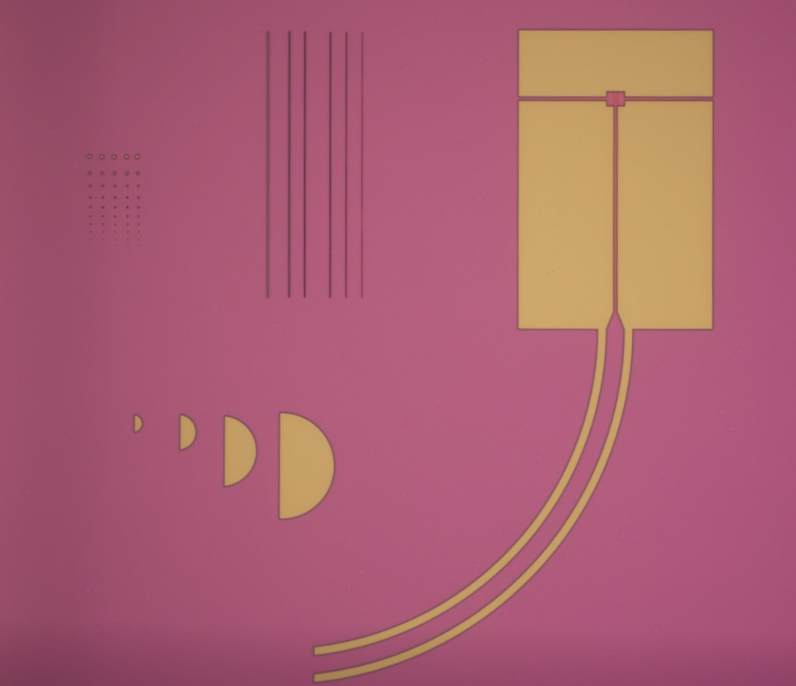
\includegraphics[width=1\textwidth]{Pic/Csar_postdev.png}
         \caption{}
         \label{}
     \end{subfigure}
     \hfill
     \begin{subfigure}[b]{0.5\textwidth}
         \centering
         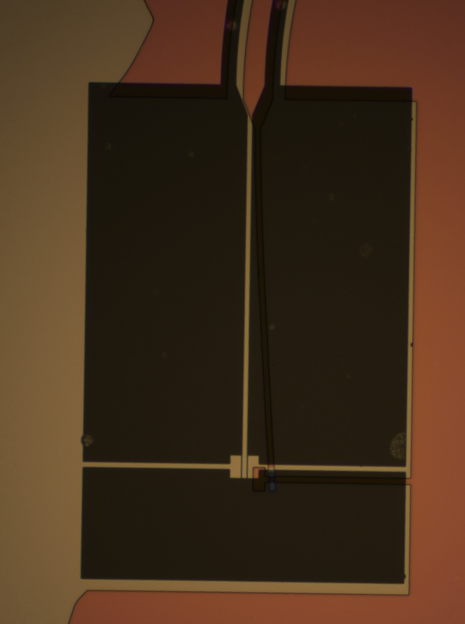
\includegraphics[width=\textwidth]{Pic/Csar_postetch_resistfall.png}
         \caption{}
         \label{}
     \end{subfigure}
    \caption{(a) The resist remains intact after the development. (b) And it falls off during the etching process after merely 8 seconds inside the acid.}
    \label{TaNWonchip2}
\end{figure}

Optical microscope can't provide enough information on how the etch looks like. We then put the chip into SEM, which shows a bad etch on the Tantalum pattern.
\clearpage
\begin{figure}[h!]
    \centering
    \begin{subfigure}[b]{0.6\textwidth}
         \centering
         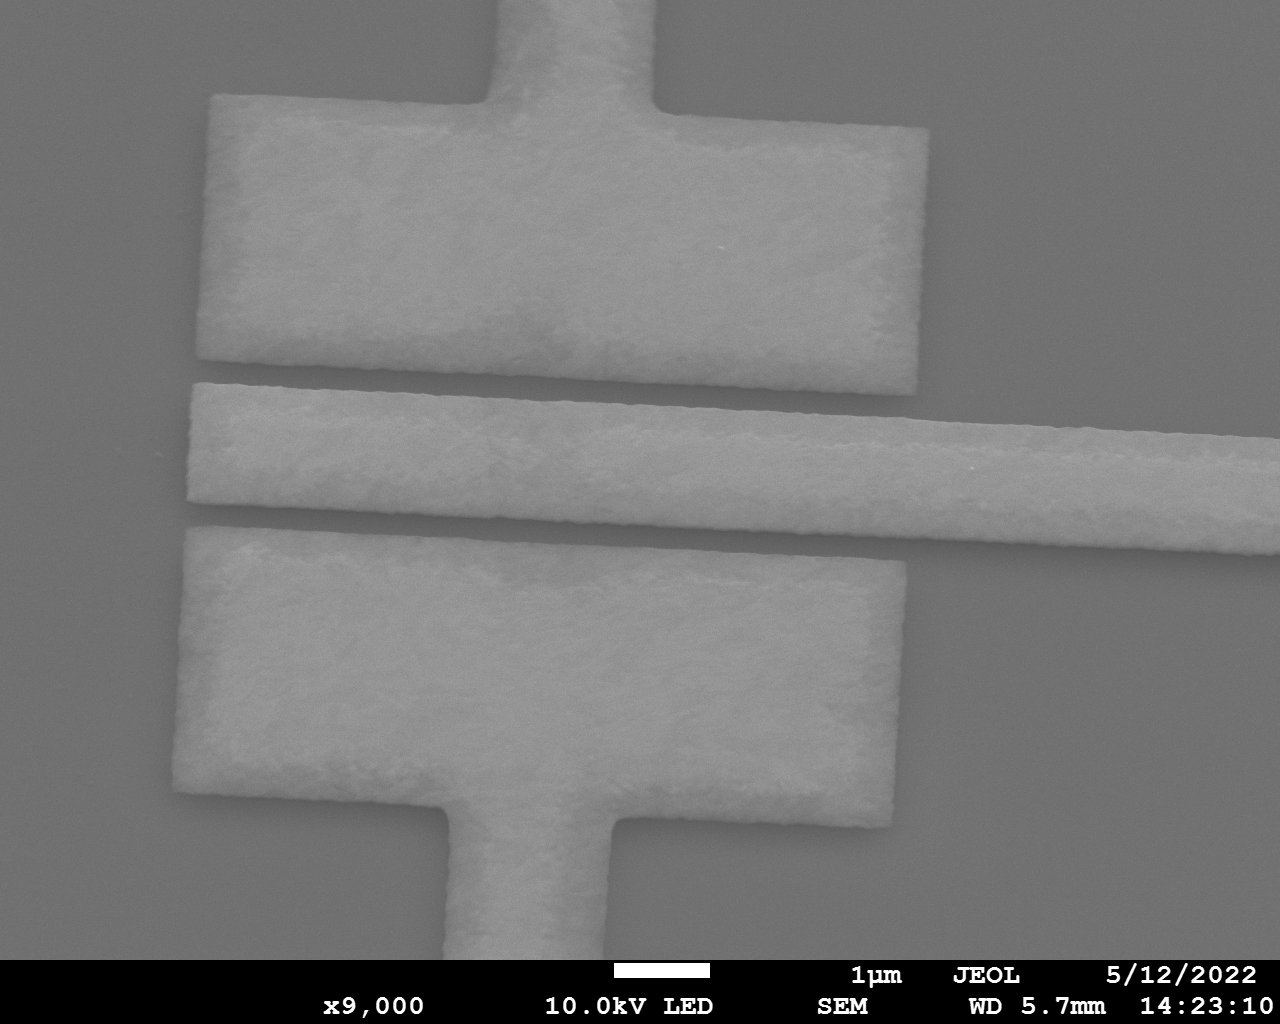
\includegraphics[width=1\textwidth]{Pic/Csar_SEM.jpg}
         \caption{}
         \label{}
     \end{subfigure}
     \hfill
     \begin{subfigure}[b]{0.6\textwidth}
         \centering
         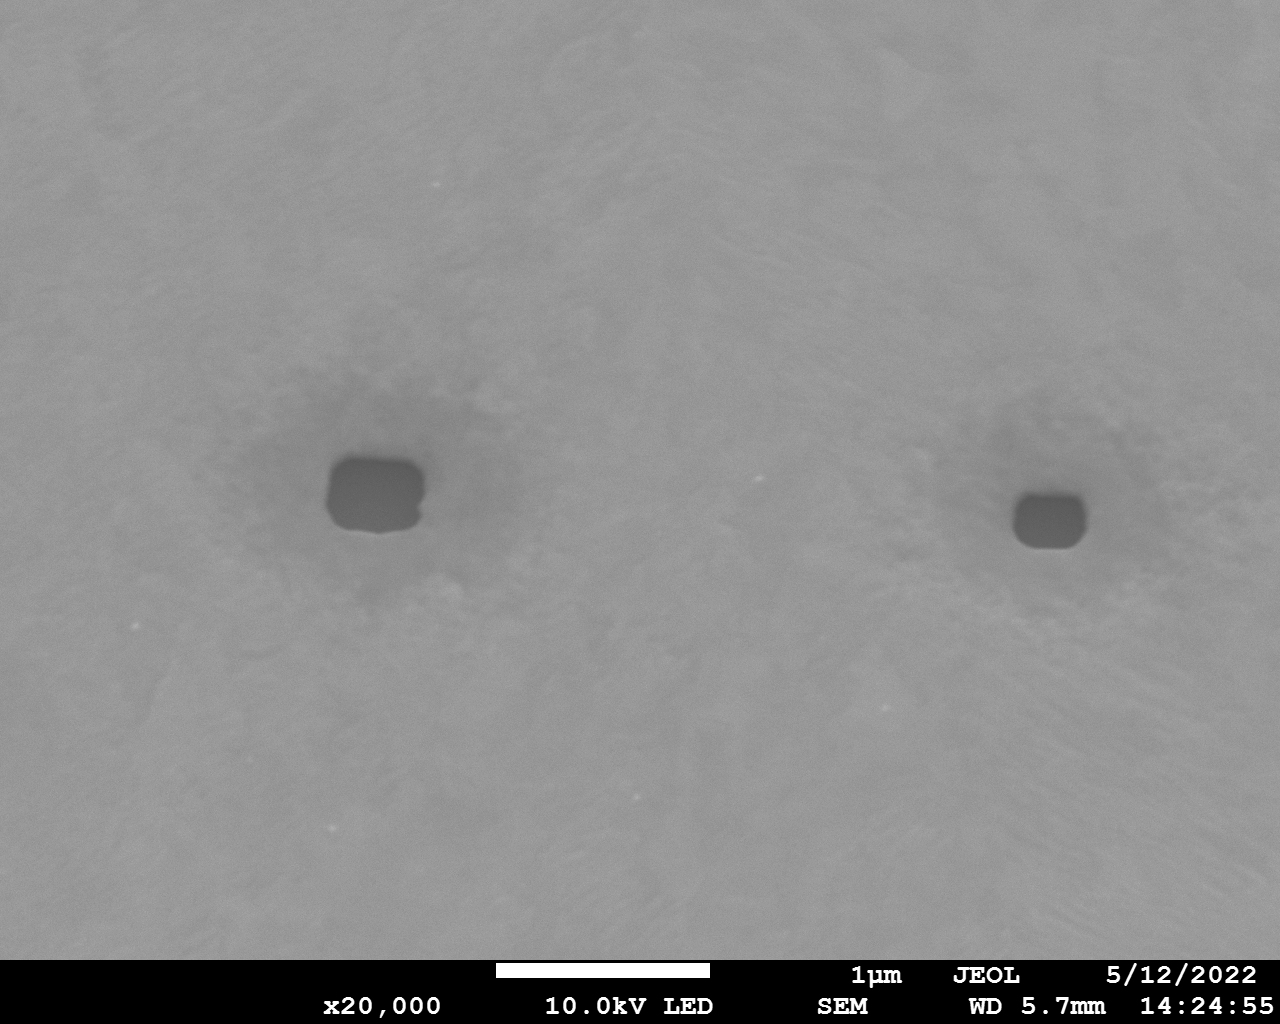
\includegraphics[width=\textwidth]{Pic/Csar_SEM_0.jpg}
         \caption{}
         \label{}
     \end{subfigure}
    \caption{The etch}
    \label{TaNWonchip2}
\end{figure}

In the SEM photos, we can clearly see the Transene 111 is attacking the Tantalum pattern surface during the etch. These evidences show that Csar 13 is not a good candidate in Tantalum wet etch with Transene 111. However, The pattern on the chip appears with sharp edge and without distortion. Therefore, one possible solution is to use Csar 62 with low spin rate, which has more than 1 $\mu m$ thickness, to do EBL.

\section{Trail on PMMA layers}

\begin{figure}[h!]
    \centering
    \begin{subfigure}[b]{0.6\textwidth}
         \centering
         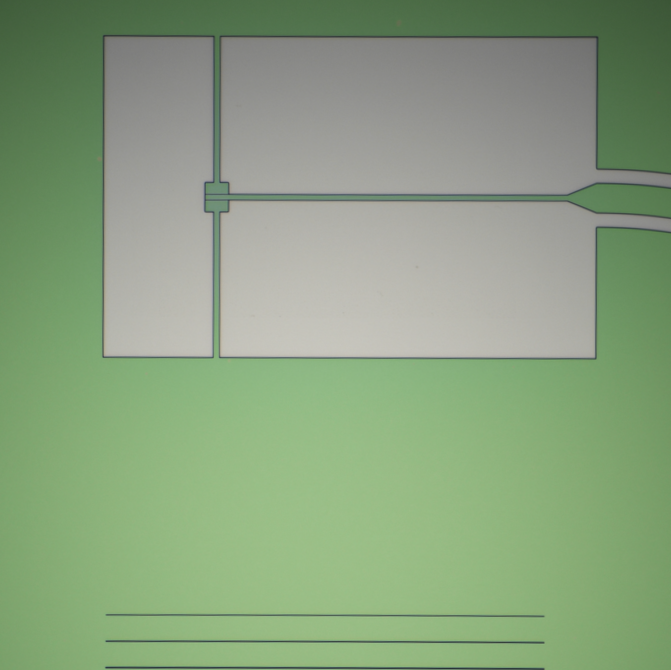
\includegraphics[width=1\textwidth]{Pic/PMMA_postdev.png}
         \caption{}
         \label{}
     \end{subfigure}
     \hfill
    \begin{subfigure}[b]{0.6\textwidth}
         \centering
         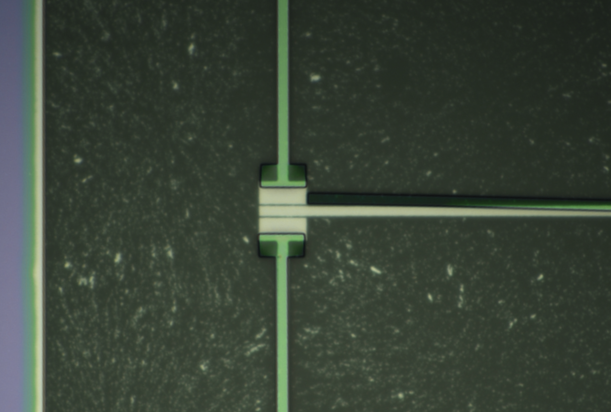
\includegraphics[width=1\textwidth]{Pic/PMMA_postetch_0.png}
         \caption{}
         \label{}
     \end{subfigure}
     \hfill
     \begin{subfigure}[b]{0.6\textwidth}
         \centering
         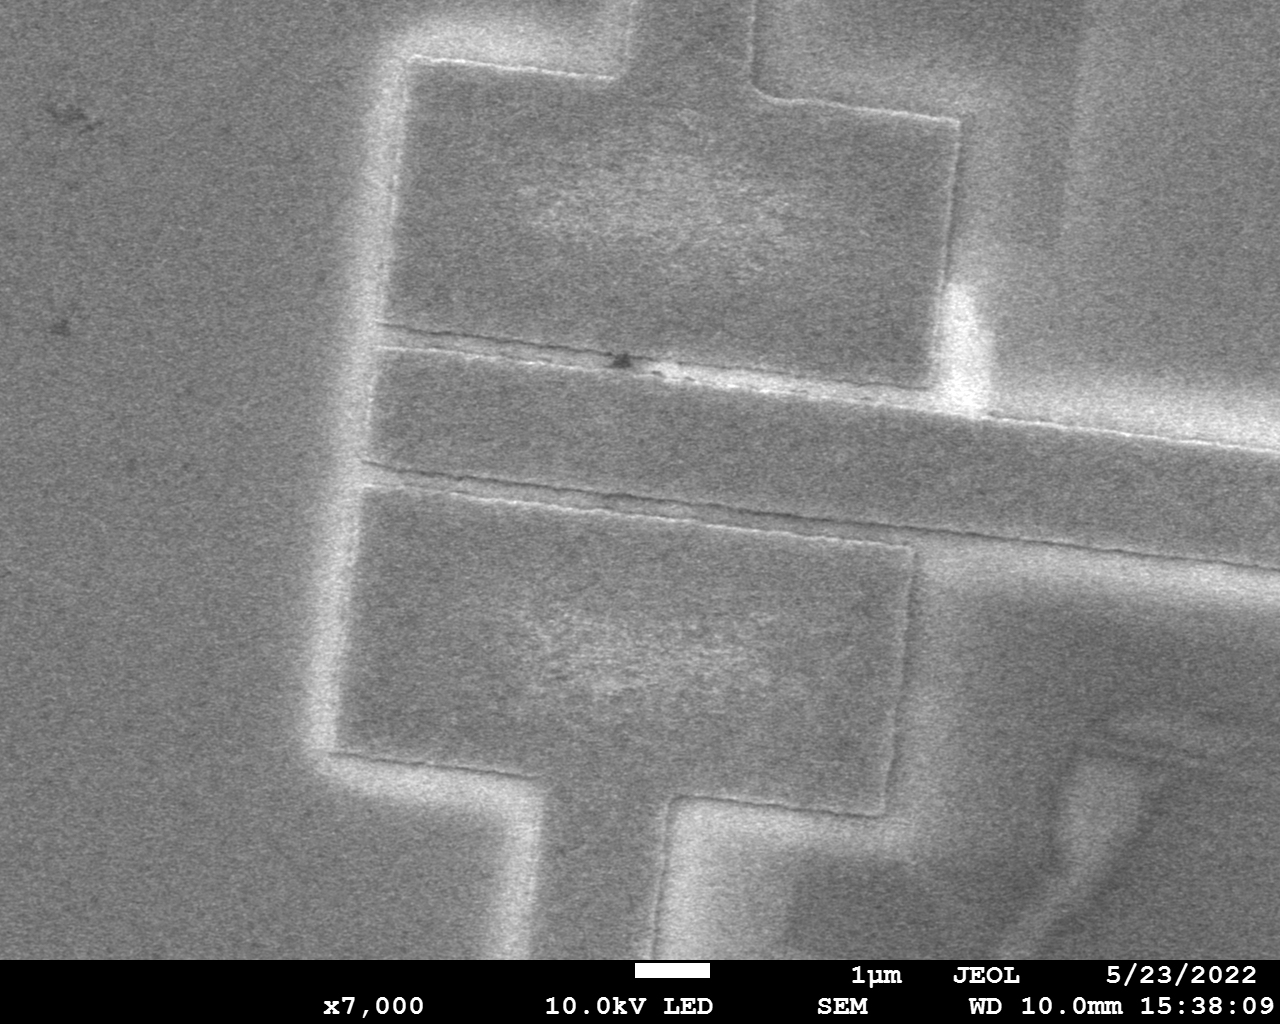
\includegraphics[width=\textwidth]{Pic/PMMA_postetch.png}
         \caption{}
         \label{}
     \end{subfigure}
    \caption{(a) After development on the PMMA. (b) The etch on the PMMA}
    \label{TaNWonchip2}
\end{figure}

PMMA series is another possible resist that we can try. We try several different combinations of PMMA recipes to thicken the resist layer:

\begin{enumerate}
    \item Pre-clean the chip 10 minutes in 1,3-dioxolane, 3 minutes in acetone with sonication, and 1 min IPA. Dry it with nitrogen.
    \item Spin PMMA A6 on the chip with 4000 rpm / 45 seconds, then bake it with 185 degree for 1 minute.
    \item Spin PMMA A6 on the chip with 4000 rpm / 45 seconds, then bake it with 185 degree for 1 minute. (Optional)
    \item Spin PMMA A2 on the chip with 4000 rpm / 45 seconds, then bake it with 185 degree for 1 minute.
    \item Lithography on ELS-F125 ebeam system with $1000\mu C  / cm^2$. Develop in MIBK:IPA (1:3) for 60 seconds, IPA for 30 seconds and dry.
    \item Ash in Diener plasma asher for 1 minute, and post-bake it for 2 minutes, 115 degree.
    \item Etch the chip in Transene 111 for 9 seconds with slow stirring (0.5Hz) and then dip it into the first MilliQ for 20 seconds, and the second MilliQ for 30 seconds.
    \item Strip it with 50 degree acetone for 10 minutes and the IPA for 1 minute. 
\end{enumerate}

The total thickness of the resist is up to 800 nm if two layers of PMMA A6 and one layer of PMMA A2 is spun on. This recipe has a similar resist falling off and distortion issue to the Csar one. Moreover, the etching always leaves some leftover Tantalum on the sapphire, even if we extend the etching time. Beyond 15 seconds, the pattern will all disappear. SEM pictures show that the surface are attacked severely, which is not ideal for the qubit devices since it might generate extra TLS coupled to the transmon system.
